\documentclass[journal,12pt,onecolumn]{IEEEtran}
\usepackage{graphicx, float}
\graphicspath{{Figs/}}
\usepackage{multicol}
\usepackage{parskip}
\usepackage{titlesec}
\usepackage{color}
\usepackage{enumitem}
\usepackage{amsmath,amssymb,amsfonts,amsthm}
\usepackage{array}
\usepackage{booktabs}
\usepackage[table]{xcolor}
\usepackage{longtable}
\usepackage{gensymb}
\usepackage{cite}
\usepackage{algorithmic}
\usepackage{textcomp}
\usepackage{txfonts}
\usepackage{listings}
\usepackage{mathtools}
\usepackage{comment}
\usepackage{tkz-euclide}
\usepackage[breaklinks=true]{hyperref}
\usepackage{gvv}
\usepackage[latin1]{inputenc}
\usetikzlibrary{arrows.meta, positioning}
\usepackage{xparse}
\usepackage{calc}
\usepackage{multirow}
\usepackage{hhline}
\usepackage{ifthen}
\usepackage{lscape}
\usepackage{tabularx}
\usepackage{circuitikz}
\usepackage{tikz}
\newtheorem{problem}{Problem}
\newtheorem{theorem}{Theorem}[section]
\newtheorem{proposition}{Proposition}[section]
\newtheorem{lemma}{Lemma}[section]
\newtheorem{corollary}[theorem]{Corollary}
\newtheorem{example}{Example}[section]
\newtheorem{definition}[problem]{Definition}
\newcommand{\BEQA}{\begin{eqnarray}}
\newcommand{\EEQA}{\end{eqnarray}}
\theoremstyle{remark}
\usepackage{pgfplots}
\pgfplotsset{compat=1.18}

\usepackage{tikz}

\title{GATE AG 2011}
\author{ai25btech11028 R.Manohar}
\begin{document}
\maketitle



\begin{enumerate}
    
\item The differential equation
\begin{align*}
  2\frac{d^{2}z}{dx^{2}} + \frac{dz}{dx} + 3y &= \sin x
\end{align*}

is considered to be ordinary, as it has
\begin{multicols}{4}
\begin{enumerate}
\item one dependent variable
\item one independent variable
\item more than one dependent variable
\item more than one independent variable
\end{enumerate}
\end{multicols}
\hfill{(GATE AG 2011)}

\item A square matrix [A] will be lower triangular if and only if ($a_{MN}$ represents an element of M$^{\text{th}}$ row and N$^{\text{th}}$ column of the matrix)
\begin{enumerate}
\item $a_{MN} = 0, \ N > M$
\item $a_{MN} = 0, \ M > N$
\item $a_{MN} \neq 0, \ M > N$
\item $a_{MN} \neq 0, \ N > M$
\end{enumerate}
\hfill{(GATE AG 2011)}

\item The metering mechanism of a seed drill is driven by the ground wheels at a velocity ratio of 1:2.  
When forward speed of the seed drill is increased from $3.0$ to $3.45$ km h$^{-1}$, the seed rate would
\begin{multicols}{4}
\begin{enumerate}
\item increase by 15\%
\item decrease by 15\%
\item decrease by 13\%
\item remain the same
\end{enumerate}
\end{multicols}
\hfill{(GATE AG 2011)}

\item A maize planter drops seeds at 0.20 m interval. The seed weight is 200 g per 1000 seeds.  
If the row to row spacing is 0.25 m, the seed rate in kg ha$^{-1}$ is
\begin{multicols}{4}
\begin{enumerate}
\item 5
\item 10
\item 20
\item 40
\end{enumerate}
\end{multicols}
\hfill{(GATE AG 2011)}

\item Which one of the following is \textbf{NOT} a towed wheel?
\begin{multicols}{4}
\begin{enumerate}
\item wheels of power tiller
\item wheels of bullock cart
\item front wheels of two wheel drive tractor
\item wheels of trailer
\end{enumerate}
\end{multicols}
\hfill{(GATE AG 2011)}

\item If the density of a fluid changes from point to point in a flow region, the flow is called
\begin{multicols}{4}
\begin{enumerate}
\item steady flow
\item non-uniform flow
\item unsteady flow
\item compressible flow
\end{enumerate}
\end{multicols}
\hfill{(GATE AG 2011)}

\item Capillary water is held in the soil due to
\begin{multicols}{4}
\begin{enumerate}
\item absorption force
\item gravitational force
\item surface tension force
\item osmotic force
\end{enumerate}
\end{multicols}
\hfill{(GATE AG 2011)}

\item The wedge storage in a river reach during the passage of a flood wave is
\begin{enumerate}
\item positive during rising phase
\item negative during rising phase
\item positive during falling phase
\item constant
\end{enumerate}
\hfill{(GATE AG 2011)}

\item The viscosity of a Newtonian fluid depends primarily on $X$ and to a lesser degree on $Y$.  
$X$ and $Y$ are
\begin{enumerate}
\item $X =$ temperature, $Y =$ flow velocity
\item $X =$ flow velocity, $Y =$ pressure
\item $X =$ temperature, $Y =$ pressure
\item $X =$ roughness of the surface across which the fluid flows, $Y =$ flow velocity
\end{enumerate}
\hfill{(GATE AG 2011)}

\item Milk is agitated in a tank with a rotating impeller. For this system: 
Let 
\begin{align*}
X = \frac{P}{\rho N^3 D^5}, \quad Y = \frac{D^2 N \rho}{\mu}, \quad Z = \frac{DN^2}{g} 
\end{align*}
where, $P$ = power imparted by the impeller to the fluid, $N$ = rate of rotation of the impeller, 
$D$ = impeller diameter, $g$ = acceleration due to gravity, $\rho$ = fluid density, and $\mu$ = fluid viscosity. 
The $X, Y, Z$ are
\begin{enumerate}
\item $X$ = Grashof number, $Y$ = Power number, $Z$ = Reynolds number  
\item $X$ = Power number,$Y$ = Reynolds number,$Z$ = Froude number 
\item $X$ = Reynolds number,$Y$ = Froude number,$Z$ = Grashof number 
\item $X$ = Froude number,$Y$ = Grashof number,$Z$ = Power number
\end{enumerate}
\hfill{(GATE AG 2011)}

\item The highest order of polynomial integrand for which Simpson's 1/3 rule of integration is exact is
\begin{multicols}{4}
\begin{enumerate}
\item first 
\item second  
\item third 
\item fourth
\end{enumerate}
\end{multicols}
\hfill{(GATE AG 2011)}

\item The mean value of a function $f(x)$ from $x=a$ to $x=b$ is given by
\begin{multicols}{2}
\begin{enumerate}
\item $\frac{f(a) + f(b)}{2}$ 
\item $\frac{\int_a^b f(x)\,dx}{b-a}$
\item $\frac{f(a) + 2f\left(\frac{a+b}{2}\right) + f(b)}{4}$ 
 \item $\int_a^b f(x)\,dx$
\end{enumerate}
\end{multicols}
\hfill{(GATE AG 2011)}

\item A statistical measure of the variability of a distribution around its mean is referred to as
\begin{multicols}{4}
\begin{enumerate}
\item coefficient of determination 
\item coefficient of variation
\item standard error 
\item standard deviation
\end{enumerate}
\end{multicols}
\hfill{(GATE AG 2011)}

\item An engine is to be run in dual fuel mode using diesel and producer gas with diesel as pilot fuel. Operation NOT required while running the engine is
\begin{multicols}{4}
\begin{enumerate}
\item cooling of the producer gas 
\item preheating of the producer gas
\item cleaning of the producer gas  
\item mixing of producer gas with air
\end{enumerate}
\end{multicols}
\hfill{(GATE AG 2011)}

\item The range of frequency of vertical vibration of tractor most harmful to the operator's body at a root mean square acceleration of 1.0 m ${s}^{-2}$ in Hertz is
\begin{multicols}{4}
\begin{enumerate}
\item 0.4-0.8 
\item 4.0-8.0  
\item 400-800 
\item 4000-8000
\end{enumerate}
\end{multicols}
\hfill{(GATE AG 2011)}

\item The Sauter mean diameter of liquid droplets of a hydraulic spray is
\begin{multicols}{4}
\begin{enumerate}
\item median diameter of droplets 
\item mean diameter of droplets 
\item surface area of droplets 
\item volume to surface area ratio of droplets
\end{enumerate}
\end{multicols}
\hfill{(GATE AG 2011)}


\item A horizontal axis windmill having 8 blades is used for pumping water. Each blade has a tip radius of 1.0 m and a mean chord of 0.1 m. Assuming blade length equal to tip radius, solidity of the windmill is
\begin{multicols}{4}
\begin{enumerate}
\item 0.03 
\item 0.10 
\item 0.25 
\item 0.80
\end{enumerate}
\end{multicols}
\hfill{(GATE AG 2011)}

\item A completely saturated clay soil has particle density of 2600 kg${ m}^{-3}$ and bulk density of 1400 kg ${m^-3}$. It has a moisture fraction of 40\% on volume basis. The porosity of the soil is
\begin{multicols}{4}
\begin{enumerate}
\item 0.46 
\item 0.54
\item 0.74 
\item 0.86
\end{enumerate}
\end{multicols}
\hfill{(GATE AG 2011)}

\item The magnetic bearing of a line at a station point is found to be $182^\circ$. 
The magnetic declination at the station is $3^\circ$ E and the local attraction is $-1^\circ$ for correction. 
The true bearing of the line is
\begin{multicols}{4}
\begin{enumerate}
\item $186^\circ$
\item $184^\circ$
\item $180^\circ$
\item $178^\circ$
\end{enumerate}
\end{multicols}
\hfill{(GATE AG 2011)}

\item In wind erosion process, the rate of soil movement (S) depends on wind speed (v), 
threshold limit of wind speed required to move the soil $(v_m)$ and average soil particle size (d). 
This interrelationship is expressed as
\begin{multicols}{4}
\begin{enumerate}
\item $S \propto (v - v_m)^2\,d^{1/2}$
\item $S \propto (v - v_m)^3\,d^{1/2}$
\item $S \propto (v - v_m)^2\,d$
\item $S \propto (v - v_m)^3\,d$
\end{enumerate}
\end{multicols}
\hfill{(GATE AG 2011)}

\item For a catchment with an area of 400 ${km}^2$, the equivalent discharge of the S-curve obtained by summation of 4-h unit hydrograph in m$^3$ s$^{-1}$ is
\begin{multicols}{4}
\begin{enumerate}
\item 100
\item 139
\item 200
\item 278
\end{enumerate}
\end{multicols}
\hfill{(GATE AG 2011)}

\item A material having thermal conductivity k insulates a spherical object of diameter d. 
The heat transfer coefficient between the insulating material and the environment is $h_0$. 
The critical thickness of insulation for maximum heat transfer rate is
\begin{multicols}{4}
\begin{enumerate}
\item $\frac{k}{2h_0} - \frac{d}{2}$
\item $\frac{2k}{h_0} - \frac{d}{2}$
\item $\frac{k}{2h_0} - d$
\item $\frac{2k}{h_0} - d$
\end{enumerate}
\end{multicols}
\hfill{(GATE AG 2011)}

\item For a mass of grain stored in a bin, the angle of internal friction of the grain is $30^\circ$. 
The ratio of normal pressure to the applied pressure within the bin is
\begin{multicols}{4}
\begin{enumerate}
\item 0.25
\item 0.33
\item 0.50
\item 1.00
\end{enumerate}
\end{multicols}
\hfill{(GATE AG 2011)}

\item In a counter current concentric tube heat exchanger, the hot fluid enters at 360 K and leaves at 340 K. 
The cooling fluid enters at 300 K and leaves at 316 K. The logarithmic mean temperature difference in K is
\begin{multicols}{4}
\begin{enumerate}
\item 17.9
\item 39.2
\item 41.9
\item 57.3
\end{enumerate}
\end{multicols}
\hfill{(GATE AG 2011)}

\item A constant heat flux of 500 W ${m^{-2}}$ is supplied to one face of a food material having a plate-like structure with a thickness of 10 mm. 
The thermal conductivity of the food material is $1.5\ \mathrm{W\,m^{-1}\,^\circ C^{-1}}$. 
From the other face of the food material, heat is dissipated by convection into a fluid of $40^\circ\mathrm{C}$ temperature. 
The heat transfer coefficient of the fluid is $100\ \mathrm{W\,m^{-2}\,^\circ C^{-1}}$. 
The temperature in $^\circ\mathrm{C}$ of the surface to which the heat flux is supplied will be
\begin{multicols}{4}
\begin{enumerate}
\item 43.3
\item 45.3
\item 48.3
\item 54.3
\end{enumerate}
\end{multicols}
\hfill{(GATE AG 2011)}

\item The stationary points of $f(x,y) = \frac13 x^3 - xy^2 - 2y$ are
\begin{multicols}{4}
\begin{enumerate}
\item $(1,-1)$ and $(-1,1)$
\item $(1,1)$ and $(-1,-1)$
\item $(2,-2)$ and $(-2,2)$
\item $(2,2)$ and $(-2,-2)$
\end{enumerate}
\end{multicols}
\hfill{(GATE AG 2011)}

\item The divergence of the vector $\mathbf{F} = \sin(xy)\,\mathbf{i} + y\cos(z)\,\mathbf{j} + xz\cos(z)\,\mathbf{k}$ 
(i, j, and k represent unit vectors along the three orthogonal axes) at $x = y = 0$ is
\begin{multicols}{4}
\begin{enumerate}
\item $\sin(z)$
\item $\cos(z)$
\item $-\sin(z)$
\item $-\cos(z)$
\end{enumerate}
\end{multicols}
\hfill{(GATE AG 2011)}

\item A plane contains the following three points: P$(2,1,5)$, Q$(-1,3,4)$ and R$(3,0,6)$.  
The vector perpendicular to the above plane can be represented as
\begin{multicols}{4}
\begin{enumerate}
\item 2i - j + k
\item i + 2j + 2k
\item 2i + 3j + k
\item i + 2j + k
\end{enumerate}
\end{multicols}
\hfill{(GATE AG 2011)}

\item The solution of 
\begin{align*}
    x \frac{dy}{dx} = x^2 + 3y
\end{align*}
for $x>0$ and $y(1)=2$ is
\begin{multicols}{4}
\begin{enumerate}
\item $y = x^3 + 3x^2$
\item $y = x^2 + 3x^3$
\item $y = -x^2 + 3x^3$
\item $y = -x^2 - 3x^3$
\end{enumerate}
\end{multicols}
\hfill{(GATE AG 2011)}

\item A two cylinder four stroke diesel engine develops $15\ \mathrm{kW}$ power at 2400 rpm.  
Its brake specific fuel consumption is $0.268\ \mathrm{kg\ kW^{-1}\ h^{-1}}$.  
If the specific gravity of fuel is $0.85$, quantity of fuel injected per cylinder per cycle in $\mathrm{m}^3$ is
\begin{multicols}{4}
\begin{enumerate}
\item $0.028 \times 10^{-6}$
\item $0.033 \times 10^{-6}$
\item $0.056 \times 10^{-6}$
\item $0.065 \times 10^{-6}$
\end{enumerate}
\end{multicols}
\hfill{(GATE AG 2011)}

\item A hydraulic spray nozzle has a discharge of $450\ \mathrm{ml\ min^{-1}}$ at a pressure of $280\ \mathrm{kPa}$.  
If the pressure is increased by $10\%$, the discharge will be
\begin{multicols}{4}
\begin{enumerate}
\item increased by 4.9\%
\item increased by 10.0\%
\item increased by 21.0\%
\item decreased by 4.6\%
\end{enumerate}
\end{multicols}
\hfill{(GATE AG 2011)}

\item In a cutter bar mower, the cutter bar drive consists of an offset slider crank mechanism with a crank of radius 36 mm and a pitman of length 360 mm.  
If offset of the crank is 72 mm, the stroke length in mm would be
\begin{multicols}{4}
\begin{enumerate}
\item 36.0
\item 72.0
\item 73.5
\item 80.5
\end{enumerate}
\end{multicols}
\hfill{(GATE AG 2011)}

\item The cost of a tractor is Rs. 340000. Its service life is 10 years and the salvage value is 10\% of initial cost.  
Its depreciation in $2^{\mathrm{nd}}$ year, following constant rate method, in rupees would be
\begin{multicols}{4}
\begin{enumerate}
\item 30600
\item 34000
\item 50070
\item 55550
\end{enumerate}
\end{multicols}
\hfill{(GATE AG 2011)}

\item The resultant soil reaction force acting on a single bottom mould board plough has a component of 1200 N acting at an angle of $31^\circ$ downwards in a vertical plane.  
This plane is along the direction of travel. Weight of the plough is 620 N.  
Neglecting the side forces, the magnitude of pull in N would be
\begin{multicols}{4}
\begin{enumerate}
\item 618
\item 1028
\item 1350
\item 1609
\end{enumerate}
\end{multicols}
\hfill{(GATE AG 2011)}

\item A concrete-lined non-circular tunnel has a semi-circle at the top and a rectangular section at the bottom.  
The semi-circle has a diameter of 6 m whereas the rectangular section is 6 m wide and 3 m high.  
The tunnel carries a discharge of 128 ${m^3\ s^{-1}}$.  
If the friction factor f=0.017, then the head loss in 1 km length of the tunnel in m will be
\begin{multicols}{4}
\begin{enumerate}
\item 0.57
\item 1.15
\item 2.29
\item 4.58
\end{enumerate}
\end{multicols}
\hfill{(GATE AG 2011)}

\item In a falling head permeameter test, the initial head is 0.30 m
The head drops to 0.01 m in 40 min.  
The permeability of a soil sample, 0.06 m high and $50\times 10^{-4}\ \mathrm{m^2}$ in cross-sectional area, is found to be $1.0\times 10^{-6}\ \mathrm{m\ s^{-1}}$.  
The size of the stand pipe in ${m^2}$ is
\begin{multicols}{4}
\begin{enumerate}
\item 1.82
\item $1.82\times 10^{1}$
\item $1.82\times 10^{-2}$
\item $1.82\times 10^{-4}$
\end{enumerate}
\end{multicols}
\hfill{(GATE AG 2011)}

\item A 100 ha reservoir receives 2500 mm of rainfall during a period of 2 years.  
During this period the mean inflow to the stream is 1.0 ${m^3\ s^{-1}}$, the mean outflow from the stream is 0.8 ${m^3\ s^{-1}}$, and the increase in the storage is 500 ha m.  
Assuming that there is no seepage loss, the total evaporation during the period in m is
\begin{multicols}{4}
\begin{enumerate}
\item 1.011
\item 10.11
\item 101.1
\item 1011
\end{enumerate}
\end{multicols}
\hfill{(GATE AG 2011)}

\item The following figure presents the hyetograph for a 3-hour storm. The surface runoff for the event is estimated to be 38 mm. The phi-index for the event in $mm h{^-1}$ is 



\begin{figure}[h!]
\centering
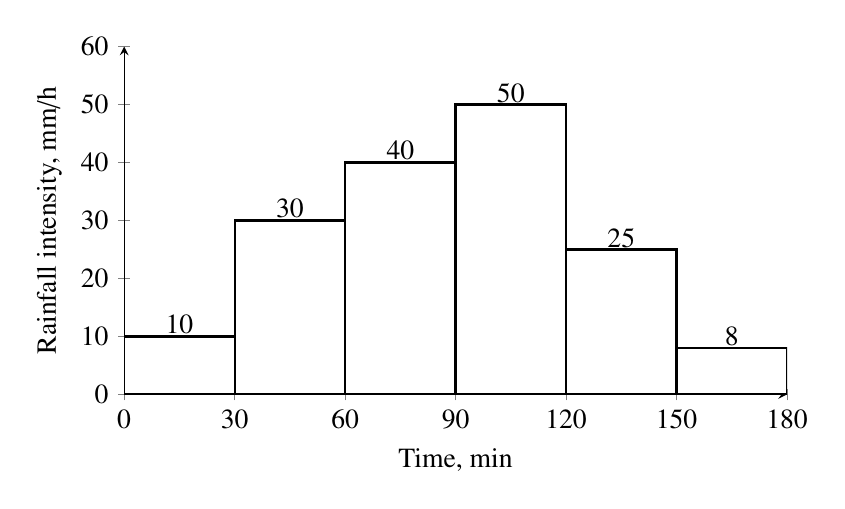
\begin{tikzpicture}
\begin{axis}[
    width=10cm,
    height=6cm,
    xlabel={Time, min},
    ylabel={Rainfall intensity, mm/h},
    ymin=0, ymax=60,
    xmin=0, xmax=180,
    xtick={0,30,60,90,120,150,180},
    ytick={0,10,20,30,40,50,60},
    axis lines=left,
    ymajorgrids=false,
    xmajorgrids=false
]

% Draw filled bars
\addplot[ybar interval, fill=white, draw=black, thick] 
coordinates {
    (0,10) (30,30) (60,40) (90,50) (120,25) (150,8) (180,8)
};

% Add intensity labels above bars
\node at (axis cs:15,12) {10};
\node at (axis cs:45,32) {30};
\node at (axis cs:75,42) {40};
\node at (axis cs:105,52) {50};
\node at (axis cs:135,27) {25};
\node at (axis cs:165,10) {8};

\end{axis}
\end{tikzpicture}
\end{figure}

\begin{multicols}{4}
\begin{enumerate}
    \item 11.50
    \item 14.25
    \item 15.80
    \item 17.25
\end{enumerate}
\end{multicols}
\hfill{(GATE AG 2011)}


\item 
A crop grown over an area of 50 ha can tolerate 5 decisiemens m$^{-1}$ of electrical conductivity in the drainage water. The consumptive use of the crop is 1.0 m, 30\% of which is obtained from the rainfall and the remainder is met from the irrigation water having electrical conductivity of 2 decisiemens m$^{-1}$. For efficient crop production, the leaching requirement and the quantity of water that must be drained from the area are
\begin{multicols}{2}
\begin{enumerate}
    \item 40\% and 0.23 Mm$^3$
    \item 60\% and 0.23 Mm$^3$
    \item 40\% and 0.21 Mm$^3$
    \item 60\% and 0.21 Mm$^3$
\end{enumerate}
\end{multicols}
\hfill{(GATE AG 2011)}

\item 
A fully penetrating tubewell of 0.2 m diameter is operational in a confined aquifer of 20 m thickness. The hydraulic conductivity of the formation ($K$) is 20 m per day and the radius of influence is 1000 m. Water table is 50 m above the bottom of screen and the maximum drawdown is 10 m. Subsequently two more tubewells of the same size are installed in such a way that the three tubewells form an equilateral triangle of side 300 m. All three tubewells have equal discharge when operated independently. If all tubewells are operated simultaneously, the percent loss in the discharge of the first well is
\begin{multicols}{4}
\begin{enumerate}
    \item 20.73
    \item 35.75
    \item 48.85
    \item 61.90
\end{enumerate}
\end{multicols}
\hfill{(GATE AG 2011)}

\item 
For the eastern Himalayan region having hill slope of 16\%, a bench terrace system is to be designed. It is found that the depth of cut for constructing the bench terrace cannot be more than 0.40 m due to the limitation of the soil depth. If a batter slope of $\frac{1}{2} : 1$ is proposed, the maximum possible width of the terrace and the required earthwork per hectare (assuming cut equal to fill) will be
\begin{multicols}{4}
\begin{enumerate}
    \item 3.4 m, 680 m$^3$
    \item 4.8 m, 960 m$^3$
    \item 4.6 m, 920 m$^3$
    \item 5.0 m, 1000 m$^3$
\end{enumerate}
\end{multicols}
\hfill{(GATE AG 2011)}

\item 
The sieve analysis of a finely ground rice powder is represented by a straight line from zero percent mass at 1 $\mu$m particle size to 100 percent mass at 101 $\mu$m particle size. The volume-surface mean diameter in $\mu$m is
\begin{multicols}{4}
\begin{enumerate}
    \item 14.6
    \item 19.2
    \item 21.7
    \item 25.3
\end{enumerate}
\end{multicols}
\hfill{(GATE AG 2011)}

\item 
A plate shaped frozen food has a thickness of 20 mm, average thermal conductivity of 2.58 W m$^{-1}$ °C$^{-1}$, density of 1080 kg m$^{-3}$, specific heat of 3550 J kg$^{-1}$ °C$^{-1}$, and a uniform temperature of $-20$ °C. The food material is suddenly immersed in a well stirred hot water maintained at a constant temperature of 90 °C. The heat transfer coefficient between the food material and hot water is 25 W m$^{-2}$ °C$^{-1}$. The time required for the centre temperature of the food material to reach 30 °C in minutes is
\begin{multicols}{4}
\begin{enumerate}
    \item 3.9
    \item 7.9
    \item 15.5
    \item 31.0
\end{enumerate}
\end{multicols}
\hfill{(GATE AG 2011)}

\item 
300 kg of parboiled and wet paddy having an initial moisture content of 28\% (dry basis) was dried in a batch type dryer. During drying operation, grain sample was drawn at regular time intervals to measure its moisture content (dry basis). It was found that the moisture content of the grain bore linear relationship with drying time till 30 minutes of drying operation at which moisture content was 22.3\%. The drying rate (kg h$^{-1}$) during this interval was
\begin{multicols}{4}
\begin{enumerate}
    \item 28.3
    \item 37.5
    \item 41.7
    \item 48.1
\end{enumerate}
\end{multicols}
\hfill{(GATE AG 2011)}

\item 
A mixture of microorganisms, P, Q, R, and S are to be inactivated by autoclaving. Number of spores of the above organisms is $6 \times 10^5$, $4 \times 10^6$, $2 \times 10^4$, and $9 \times 10^5$ respectively. Further, their decimal reduction time ($D$) values in minute are 2.2, 1.8, 0.8, and 1.6 respectively. It is desired to microbiologically inactivate the mixture at 121$^\circ$C to obtain a probability of spoilage of $10^{-5}$. The microorganisms that will be inactivated first and that at the last are respectively
\begin{multicols}{4}
\begin{enumerate}
    \item P and Q
    \item R and P
    \item P and S
    \item P and R
\end{enumerate}
\end{multicols}
\hfill{(GATE AG 2011)}

\item 
The average interstitial velocity in a packed bed is 2.5 m s$^{-1}$ and the superficial velocity under minimum fluidized condition based on the cross-section of the empty container is 1 m s$^{-1}$. Solid particles having density of 1200 kg m$^{-3}$ and size of 0.15 mm are to be fluidized using air at 3 atm absolute pressure and 30$^\circ$C temperature having a density of 3.5 kg m$^{-3}$. The empty bed cross section is 0.4 m$^2$ and the bed contains 400 kg of solid. Pressure drop at minimum fluidized condition in Pa is
\begin{multicols}{4}
\begin{enumerate}
    \item $3.5 \times 10^3$
    \item $6.5 \times 10^3$
    \item $9.7 \times 10^3$
    \item $17.1 \times 10^3$
\end{enumerate}
\end{multicols}
\hfill{(GATE AG 2011)}

\item 
Sphericity of a particle is defined as: (surface to volume ratio for a sphere having identical volume as that of the particle) / (the surface to volume ratio of the particle). The measure of sphericity of a cube shaped sugar crystal is
\begin{multicols}{4}
\begin{enumerate}
    \item $\left( \frac{\pi}{6} \right)^{\frac13}$
    \item $\left( \frac{\pi}{6} \right)^{\frac23}$
    \item $\left( \frac{\pi}{4} \right)^{\frac13}$
    \item $\left( \frac{\pi}{4} \right)^{\frac23}$
\end{enumerate}
\end{multicols}
\hfill{(GATE AG 2011)}

\textbf{Common Data Questions}
\textbf{Common Data for Questions 48 and 49:}

A 5 ha field under wheat crop is irrigated at 40\% depletion of available moisture content. The field capacity, wilting point and bulk density of the soil in the field are 32\% (on weight basis), 20\% (on weight basis) and 1400 kg m$^{-3}$ respectively. To irrigate the field in a day of 10 hours, a pump is used which lifts 270 m$^3$ of water per hour against a total head of 20 m.

\item 
If the root zone depth is 0.8 m, the volume of water required to irrigate the field in m$^3$ will be
\begin{multicols}{4}
\begin{enumerate}
    \item 2700
    \item 3150
    \item 3600
    \item 4050
\end{enumerate}
\end{multicols}
\hfill{(GATE AG 2011)}

\item 
The pump is driven by an electric motor. If the pump, drive and motor efficiencies are 80\%, 82\% and 90\% respectively, the required size of electric motor in horse-power will be
\begin{multicols}{4}
\begin{enumerate}
    \item 20.0
    \item 24.5
    \item 30.0
    \item 33.5
\end{enumerate}
\end{multicols}
\hfill{(GATE AG 2011)}


\textbf{Common Data for Questions 50 and 51:}

A vertical hydraulic cylinder having an inside diameter of 100 mm is used in a hoist for lifting load. 
A constant flow rate pump capable of delivering 12 litre per minute at a maximum pressure of 18 MPa is used for supplying the fluid. 
Volumetric and mechanical efficiencies of the pump are 91\% and 85\% respectively.

\item The rate of lifting of load in m s$^{-1}$ and maximum amount of load that can be lifted in kN are
\begin{multicols}{4}
\begin{enumerate}
    \item 0.020, 180
    \item 0.025, 141
    \item 0.064, 45
    \item 0.080, 565
\end{enumerate}
\end{multicols}
\hfill{(GATE AG 2011)}



\item The size of motor required for operating the pump in kW is
\begin{multicols}{4}
\begin{enumerate}
    \item 3.60
    \item 3.96
    \item 4.24
    \item 4.65
\end{enumerate}
\end{multicols}
\hfill{(GATE AG 2011)}

\textbf{Linked Answer Questions}

\textbf{Statement for Linked Answer Questions 52 and 53:}

A towed pneumatic wheel (width to diameter ratio of 0.3) is to be rolled on a leveled concrete surface. 
Total wheel load is 2000 N.


\item The force in N required to roll the wheel on the horizontal concrete surface would be
\begin{multicols}{4}
\begin{enumerate}
    \item 80
    \item 91
    \item 800
    \item 912
\end{enumerate}
\end{multicols}
\hfill{(GATE AG 2011)}



\item The minimum slope in degrees of the concrete surface with respect to the horizontal at which the wheel itself will start rolling downward is
\begin{multicols}{4}
\begin{enumerate}
    \item 2.29
    \item 5.28
    \item 23.58
    \item 27.13
\end{enumerate}
\end{multicols}
\hfill{(GATE AG 2011)}

\textbf{Statement for Linked Answer Questions 54 and 55:}

A vegetable with 70\% moisture (wet basis) is to be dried in a countercurrent dryer to give a product with 5\% moisture (wet basis). 
The feed rate to the dryer is 0.15 kg s$^{-1}$. 
The drying medium consists of air at 100$^{\circ}$C containing water vapour with a partial pressure of 1.0 kPa. 
The air leaves the dryer at 40$^{\circ}$C and is 70\% saturated. 
The system works under a total pressure of 101.3 kPa. 
The vapour pressure of water that saturates air at 40$^{\circ}$C is 7.4 kPa. 
Molecular weight of water and air may be taken as 18 and 29 respectively.



\item The humidity (kg of water vapour / kg of dry air) of the outlet air is
\begin{multicols}{4}
\begin{enumerate}
    \item 0.0027
    \item 0.0172
    \item 0.0335
    \item 0.0483
\end{enumerate}
\end{multicols}
\hfill{(GATE AG 2011)}



\item The flow rate (kg s$^{-1}$) of inlet air required is
\begin{multicols}{4}
\begin{enumerate}
    \item 0.161
    \item 0.817
    \item 1.634
    \item 3.783
\end{enumerate}
\end{multicols}
\hfill{(GATE AG 2011)}


\subsection*{General Aptitude (GA) Questions}



\subsubsection*{Q. 56 -- Q. 60 carry one mark each}

\item Choose the most appropriate word from the options given below to complete the following sentence:  
Under ethical guidelines recently adopted by the Indian Medical Association, human genes are to be manipulated only to correct diseases for which \_\_\_\_\_ treatments are unsatisfactory.


\begin{enumerate}
\item similar
\item most
\item uncommon
\item available
\end{enumerate}
\hfill{(GATE AG 2011)}




\item Choose the word from the options given below that is most nearly opposite in meaning to the given word:Frequency

\begin{enumerate}
\item periodicity
\item rarity
\item gradualness
\item persistency
\end{enumerate}
\hfill{(GATE AG 2011)}

\item Choose the most appropriate word from the options given below to complete the following sentence:  
It was her view that the country's problems had been \_\_\_\_\_ by foreign technocrats, so that to invite them to come back would be counter-productive.
\begin{multicols}{4}
\begin{enumerate}
\item identified
\item ascertained
\item exacerbated
\item analysed
\end{enumerate}
\end{multicols}
\hfill{(GATE AG 2011)}

\item There are two candidates P and Q in an election. During the campaign, 40\% of the voters promised to vote for P, and rest for Q. However, on the day of election 15\% of the voters went back on their promise to vote for P and instead voted for Q. 25\% of the voters went back on their promise to vote for Q and instead voted for P. Suppose, P lost by 2 votes, then what was the total number of voters?
\begin{multicols}{4}
\begin{enumerate}
\item 100
\item 110
\item 90
\item 95
\end{enumerate}
\end{multicols}
\hfill{(GATE AG 2011)}

\item The question below consists of a pair of related words followed by four pairs of words. Select the pair that best expresses the relation in the original pair:  
Gladiator : Arena

\begin{enumerate}
\item dancer : stage
\item commuter : train
\item teacher : classroom
\item lawyer : courtroom
\end{enumerate}
\hfill{(GATE AG 2011)}


\subsubsection*{Q. 61 -- Q. 65 carry two marks each}


\item The sum of $n$ terms of the series $4 + 44 + 444 + \dots$ is  

\begin{enumerate}
\item $\frac{4}{81} \left[10^{n+1} - 9n - 1\right]$
\item $\frac{4}{81} \left[10^{n+1} - 9n - 1\right]$
\item $\frac{4}{81} \left[10^{n+1} - 9n - 10\right]$
\item $\frac{4}{81} \left[10^{n} - 9n - 10\right]$
\end{enumerate}
\hfill{(GATE AG 2011)}


\item Given that $f(y) = \left| y \right| / y$, and $q$ is any non-zero real number, the value of $\left[ f(q) - f(-q) \right]$ is  
\begin{multicols}{4}
\begin{enumerate}
\item 0
\item $-1$
\item 1
\item 2
\end{enumerate}
\end{multicols}
\hfill{(GATE AG 2011)}

\item Three friends, R, S and T shared toffee from a bowl. R took $\frac{1}{3}$ of the toffees, but returned four to the bowl.  
S took $\frac{1}{4}$ of what was left but returned three toffees to the bowl.  
T took half of the remainder but returned two back into the bowl.  
If the bowl had 17 toffees left, how many toffees were originally there in the bowl?

\begin{multicols}{4}
\begin{enumerate}
\item 38
\item 31
\item 48
\item 41
\end{enumerate}
\end{multicols}
\hfill{(GATE AG 2011)}

\item The fuel consumed by a motorcycle during a journey while traveling at various speeds is indicated in the graph below.  




\begin{tikzpicture}[scale=0.09]

% Axes
\draw[thick] (0,0) -- (90,0); % X-axis
\draw[thick] (0,0) -- (0,120); % Y-axis

% X ticks and labels
\foreach \x in {0,15,30,45,60,75,90} {
    \draw[thick] (\x,0) -- (\x,-2);
    \node[below] at (\x,0) {\x};
}

% Y ticks and labels
\foreach \y in {0,30,60,90,120} {
    \draw[thick] (0,\y) -- (-2,\y);
    \node[left] at (0,\y) {\y};
}

% Labels
\node[below=10pt] at (45,-10) {Speed};
\node[below=24pt] at (45,-20) {(kilometres per hour)};
\node[rotate=90] at (-20,60) {Fuel consumption};
\node[rotate=90] at (-34,60) {(kilometres per litre)};

% Plot lines
\draw[thick] (10,30) -- (15,60) -- (45,90) -- (75,70);

% Data points
\foreach \x/\y in {10/30, 15/60, 45/90, 75/70} {
    \fill (\x,\y) circle (3);
}

\end{tikzpicture}



\item The distances covered during four laps of the journey are listed in the table below:  

\begin{center}
\begin{tabular}{|c|c|c|}
\hline
\textbf{Lap} & \textbf{Distance (kilometres)} & \textbf{Average speed (kilometres per hour)} \\
\hline
P & 15 & 15 \\
Q & 75 & 45 \\
R & 40 & 75 \\
S & 10 & 10 \\
\hline
\end{tabular}
\end{center}


From the given data, we can conclude that the fuel consumed per kilometre was least during the lap:  

\begin{enumerate}
\item P
\item Q
\item R
\item S
\end{enumerate}
\hfill{(GATE AG 2011)}

\item The horse has played a little known but very important role in the field of medicine. 
Horses were injected with toxins of diseases until their blood built up immunities. Then a serum was made from their blood. Serums to fight with diphtheria and tetanus were developed this way.  

It can be inferred from the passage, that horses were:  

\begin{enumerate}
\item given immunity to diseases
\item generally quite immune to diseases
\item given medicines to fight toxins
\item given diphtheria and tetanus serums
\end{enumerate}
\hfill{(GATE AG 2011)}


\begin{center}
\textbf{END OF THE QUESTION PAPER}
\end{center}






\end{enumerate}


\end{document}
